%--------Métricas
%--------Daniel Quinteros Céspedes
%--------23-09-2014

\chapter{Proceso de evaluación}
\label{cap:eval}

En los capítulos anteriores se revisó el funcionamiento tanto del proceso de extracción de características como del proceso de clasificación. El paso siguiente corresponde al proceso a través del cual se realizó la evaluación de la sensibilidad espacial. A continuación se muestra cada estapa del proceso de evaluación en general y los resultados obtenidos. Uno de los elementos relevantes es la exposición del proceso de entrenamiento de los parámetros de un sigmoide que luego permitirá transformar las salidas a probabilidades, adoptando el método propuesto por \cite{Platt1999}.

\section{Estapas del proceso de evaluación}
\label{eval:metodologia}

Para realizar la evaluación de la sensibilidad espacial se  etapas que permitiera la obtención y recolección de los resultados que conforman las matrices de sensibilidad espacial, además de la posterior evaluación utilizando la métrica propuesta en el capítulo~\ref{cap:metricas}. Los  pasos definidos son lo siguientes.

\begin{itemize}
\item Preprocesamiento de datos. El set de datos INRIA trae por defecto conjuntos de prueba y entrenamiento en tamaño original y normalizado a 64x128px por lo que fue necesario escalar las imágenes para generar conjuntos de entrenamiento en otras escalas.
\item Extracción de características. Se realizó la extracción de características para las ocho escalas diferentes generando igual número de matrices de vectores de características.
\item Entrenamiento de los clasificadores. Utilizó las matrices de características y los valores de las etiquetas de cada clase peatón y no-peatón.
\item Entrenamiento del sigmoide. En conjunto con el entrenamiento de cada clasificador, se entrenó el sigmoide mencionado antes utilizando el método de \cite{Platt1999} con la mejora matemática realizada por \cite{Lin2000}
\item Detección en la vecindad. Utilizando un enfoque de detección basado en la ventana deslizante. Se realizó el proceso de clasificación exhaustiva para toda la vecindad del conjunto obteniendo matrices con todos los valores resultantes.
\item Mapeo a probabilidades. Utilizando la ecuación (\ref{eq:sigmoid}) propuesta por \cite{Platt1999} y los valores de las constantes en el paso uno. Se mapeó cada valor de cada una de las matrices en probabilidades.
    
\begin{equation}
\centering
\label{eq:sigmoid}
P(y=1|f)=\frac{1}{1+exp(Af+B)}
\end{equation}

\item Cálculo de sensibilidad espacial. Como etapa final se realizó el cálculo de la sensibilidad promedio de los modelos resultantes además de la desviación estándar de la sensibilidad espacial para una mejor caracterización. Adicionalmente se generaron gráficas 3D que permiten observar el comportamiento de la sensibilidad espacial.
\end{itemize}

Es importante conocer el proceso en detalle por lo que se analizará cada etapa por separados. Sin embargo, para el proceso de extracción de características y el de entrenamiento de los modelo sólo se mostrarán algunos elementos adicionales relevantes pues ya fueron explicados anteriormente en las secciones~\ref{caract:seleccion} y \ref{clasificadores:seleccion} respectivamente.

\subsection{Preprocesamiento de datos}

El contenido del set de datos INRIA incluye imágenes de peatones separadas en seis conjuntos de datos diferentes, ya que tanto el conjunto de imágenes con ejemplos positivos de la clase``peatón'' que corresponde al entrenamiento, como el que corresponde a pruebas se encuentran en dos escalas diferentes: la escala con tamaño original y una escala normalizada en 64x128px. Por otra parte el conjunto de la clase ``no-peatón'' se encuentra solo en tamaño original tanto para entrenamiento como para pruebas. 

\begin{figure}[htc]
  \centering
  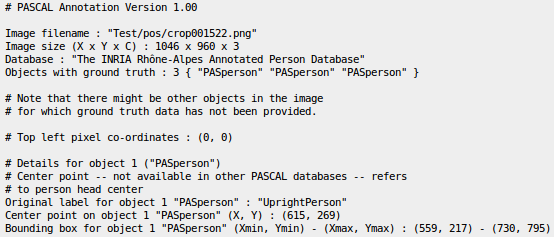
\includegraphics[scale=.6]{images/ejanotacion}
  \caption{\em Ejemplo de anotaciones incluidas en el set de datos INRIA, incluyen el centro de la cabeza y una caja alrededor de la persona a cuerpo completo }  
  \label{fig:ejanotacion}
\end{figure}

Parte importante del análisis, es la comparación en diferentes escalas, por lo que se hace necesario transformar tanto el conjunto de entrenamiento como el de test a las escalas utilizada en la comparación. Estas escalas son 32x64px, 64x128px (original normalizada), 128x256px, 256x512px. Para poder realizar esta tarea es necesario conocer de antemano la posición de la persona en la imagen, ya que es necesario centrar cada imagen en ella. En las anotaciones que vienen con set de datos (figura~\ref{fig:ejanotacion}) están incluidas las coordenadas de un rectángulo contenedor de cada persona. Para realizar este proceso se construyó un rutina en C++ que automatiza el proceso de lectura de las anotaciones y luego escala y recorta cada imagen generando un nuevo conjunto en cada uno de los tamaños antes indicados más un pequeño borde extra para evitar problemas con los bordes.

\begin{figure}[htc]
  \centering
  
\includegraphics[scale=.3]{images/32}
  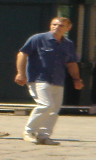
\includegraphics[scale=.3]{images/64}
  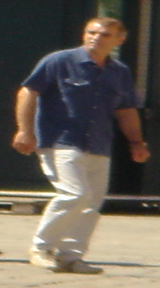
\includegraphics[scale=.3]{images/128}
  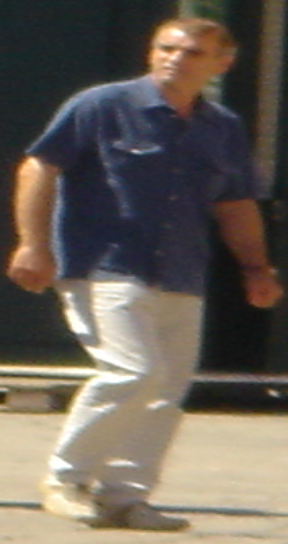
\includegraphics[scale=.3]{images/256}
  \caption{\em Imágenes  del set de datos escaladas a los tamaños utilizados, de izquierda a derecha 32x64px, 64x128px, 128x256px, 256x512px}  
  \label{fig:imgescalas}
\end{figure}

A modo de ilustración de las diferencias de tamaño entre las imágenes se expone un escalado proporcional que se puede apreciar en la figura~\ref{fig:imgescalas}.

\subsection{Extracción de características}

El proceso extracción de características ya fue explicado anteriormente en la sección \ref{caract:extraccion}, sin embargo, es importante ilustrar algunos de los resultados obtenidos en este proceso. Luego de aplicar el algoritmo HOG a cada imagen obtenemos un vector de características los que son acumulados en una matriz de características, las dimensiones de esta matriz varían según la cantidad de ejemplos y el tamaño de la ventana de clasificación utilizado.

\subsection{Entrenamiento de los clasificadores}

Para realizar el entrenamiento de los modelos de los clasificadores se utilizó la matriz de vectores de características y además los valores de etiqueta de clase. En OpenCV se sugiere utilizar para el problema de clasificación binaria valores de etiqueta 1 y -1 los cuales fueron utilizados para indicar la pertenencia a la clase ``peatón'' y ``no-peatón'' respectivamente. 

\begin{figure}[htc]
  \centering
  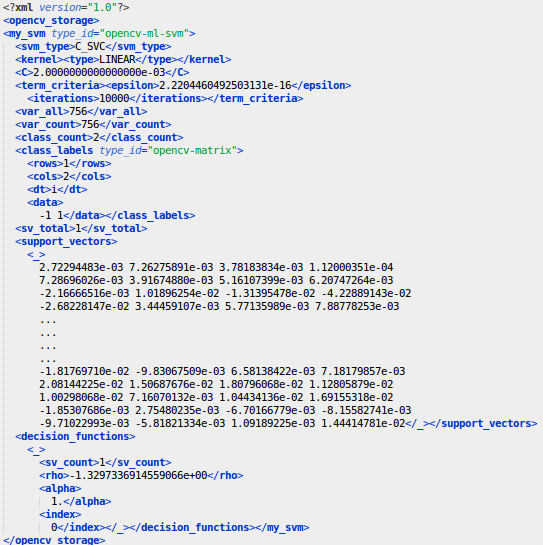
\includegraphics[scale=.6]{images/modelo}
  \caption{\em Archivo ejemplo xml con el modelo de un clasificador SVM lineal }  
  \label{fig:ejmodelo}
\end{figure}

Como resultado del entrenamiento se obtiene un modelo del clasificador almacenado en un archivo xml como el que se expone en la figura~\ref{fig:ejmodelo} 

\subsection{Entrenamiento del sigmoide}

Luego de entrenar los clasificadores es necesario realizar la normalización de las salidas de los clasificadores, para esto se utilizó un método propuesto por \cite{Platt1999}, quien indica que es posible transformar la salida de un clasificador SVM sin necesidad de utilizar un método de regularización de la máxima verosimilitud; el cual modificaría el entrenamiento del clasificador. El método planteado por Platt trata sobre el entrenamiento de los parámetros de un sigmoide adicional el cual a través de la ecuación~\ref{eq:sigmoid} transforma la salida del clasificador a probabilidades. El método de Platt es un método antiguo, pero tiene la ventaja de permitir su extensión directa a otro tipo de clasificadores no SVM como en al caso de Adaboost \citep{Niculescu-mizil2005}, si modificaciones del algoritmo. 

\begin{figure}[htc]
  \centering
  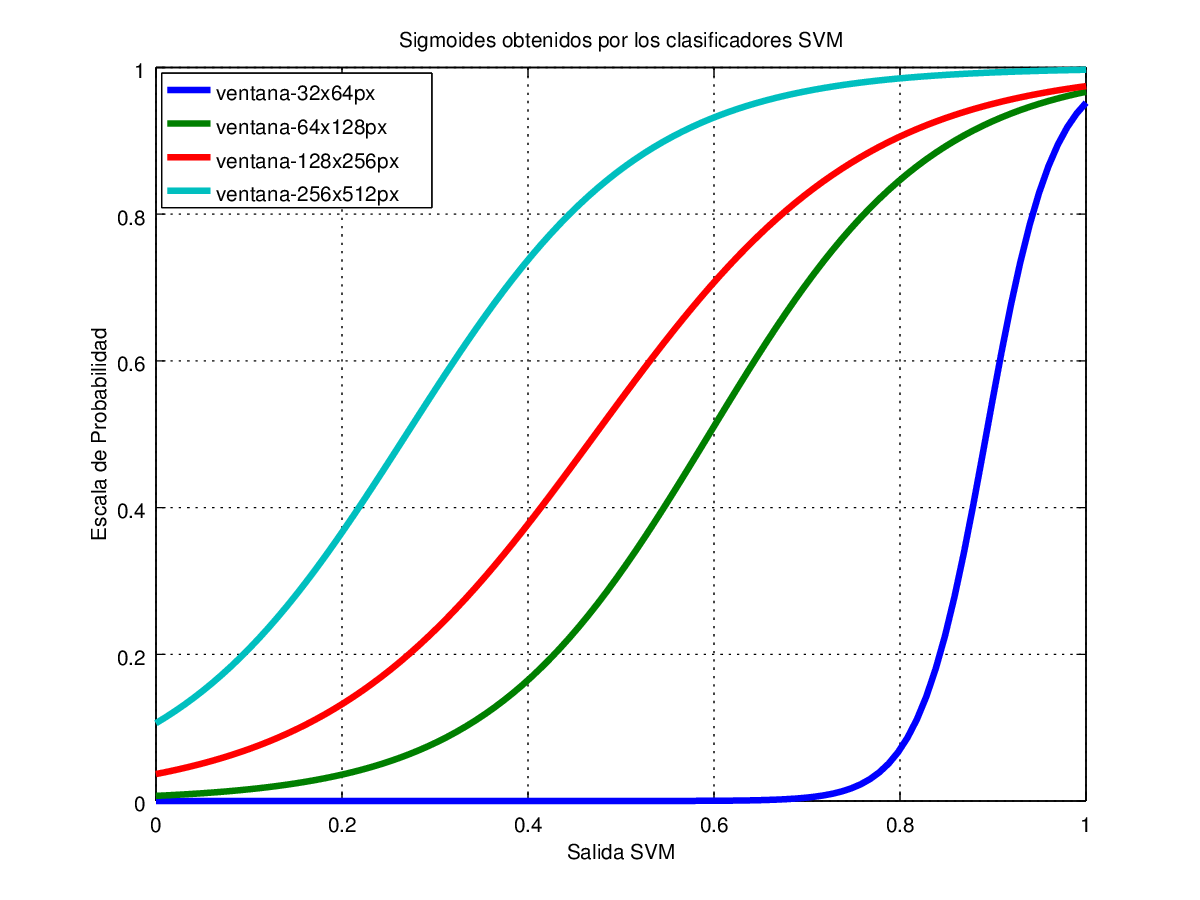
\includegraphics[scale=.4]{images/svmsig}
  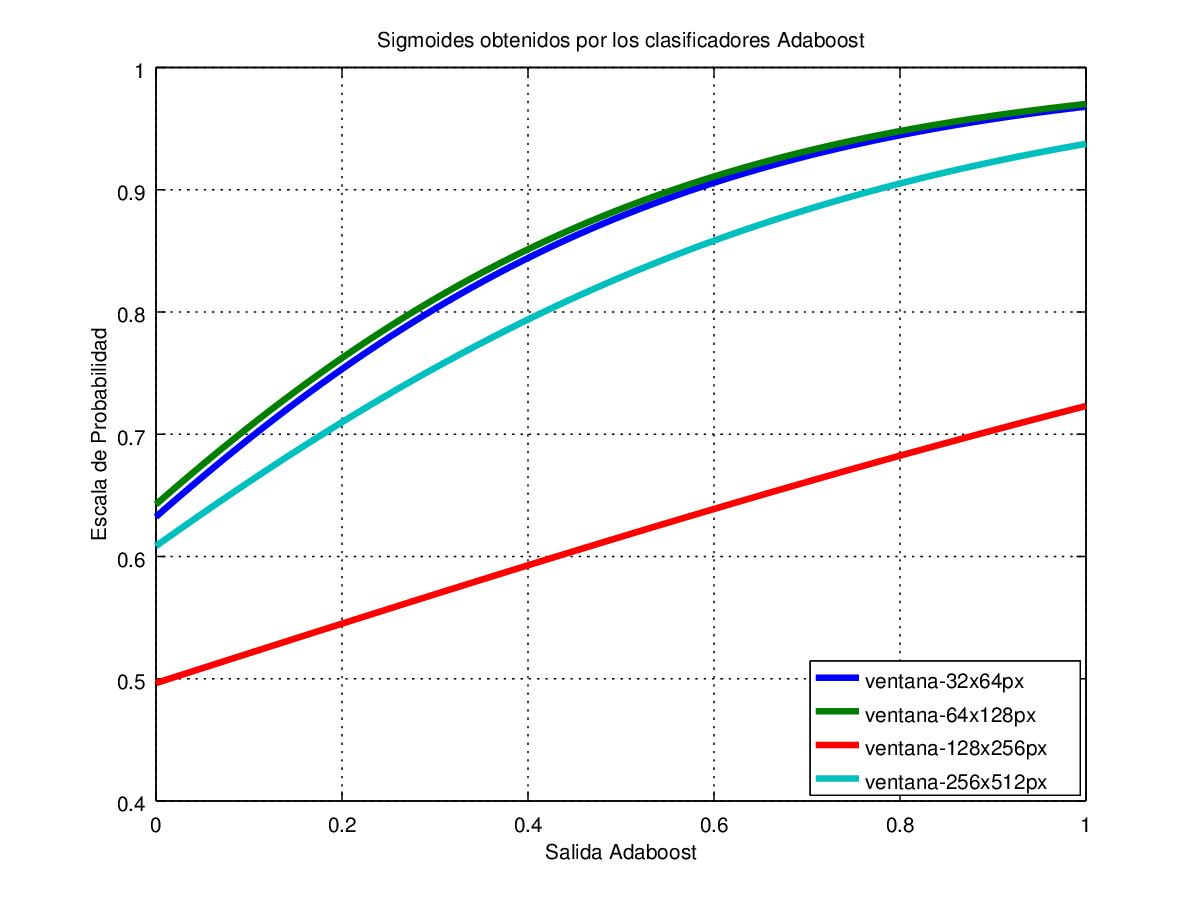
\includegraphics[scale=.4]{images/boostsig}
  \caption{\em Gráficos de los sigmoide obtenidos con el entrenamiento de los parámetros A y B de la ecuación~\ref{eq:sigmoid}}  
  \label{fig:sigmoids}
\end{figure}


% ***SAV esto es lo que quisiste decir antes sobre usar el mismo set de entrenamiento?
Para el entrenamiento es necesario tener un set de datos que consiste en ejemplos de la salida del clasificador y las etiquetas de la clase. Platt indica que se pueden obtener buenos resultados utilizando el mismo set de entrenamiento que se utilizó para entrenar el clasificador original, por lo que fue necesario realizar la evaluación con cada clasificador de cada imagen utilizada para el entrenamiento. Como previo a esto se habían calculado los descriptores HOG para estas imágenes, se mantuvo esta información en memoria durante el entrenamiento de los modelos para utilizarla en este paso.

Finalmente se obtienen los valores de las constantes A y B y los sigmoides que se pueden observar en la figura~\ref{fig:sigmoids}. Cabe notar que el algoritmo que se utilizó para el cálculo no fue exactamente el presentado por Platt en 1999 sino una mejora propuesta un año después por \cite{Lin2000}, la cual evita algunos problemas matemáticos, aumentando la robustez del algoritmo.

\subsection{Detección en la vecindad}

Una vez completadas todas las etapas de entrenamiento se utilizó un enfoque de ventana deslizante exhaustiva (prácticamente fuerza bruta) con el fin de obtener los valores para toda la vecindad (pixel a pixel) de la persona a detectar. Esto se realizó para cada imagen en el set de datos que luego de la transformación de tamaño correspondía con el tamaño de ventana del modelo evaluado.  

Las detecciones realizadas entregan como resultado una matriz con los valores de salida por cada imagen analizada. Los gráficos de estas matrices sin normalizar son como se muestran en la figura \ref{fig:rawoutput} 

\begin{figure}[htc]
  \centering
  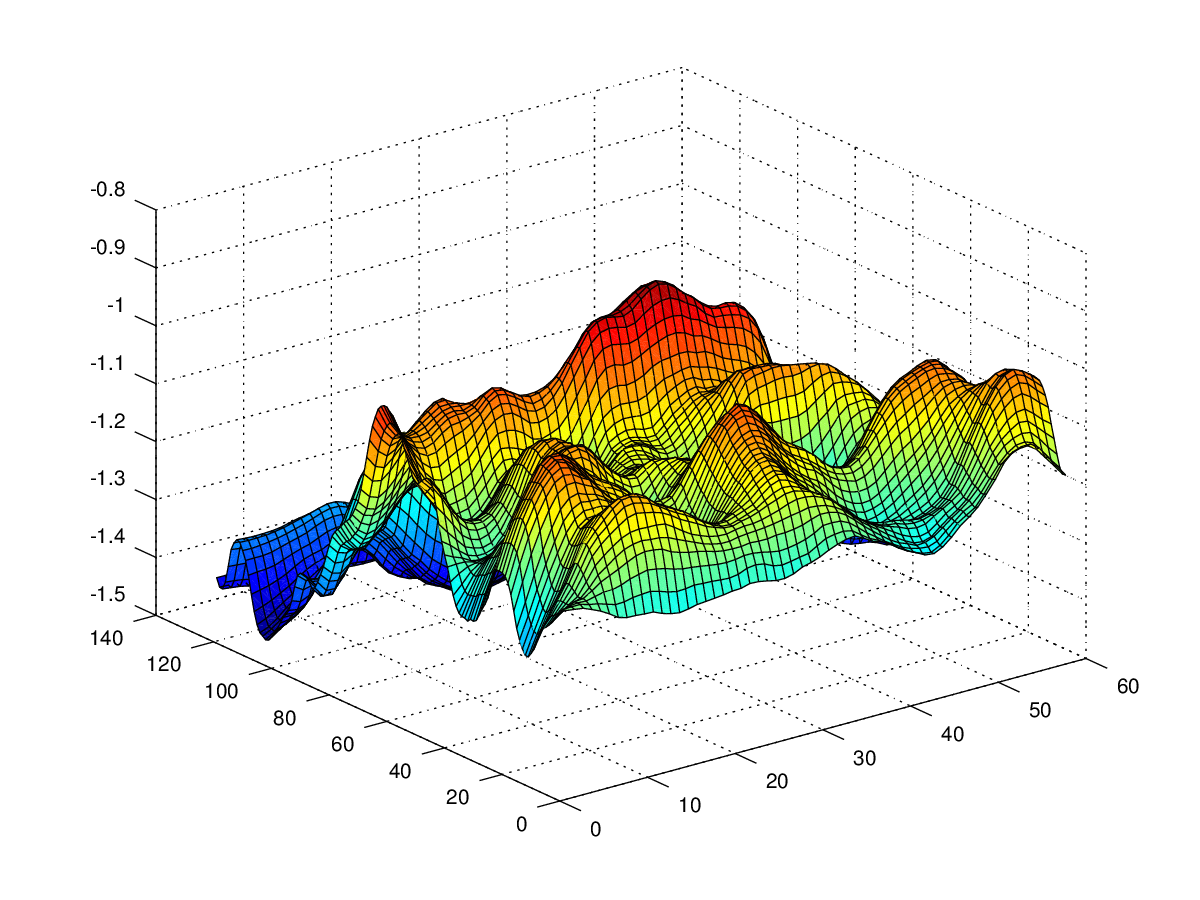
\includegraphics[scale=.3]{images/svmrawoutput}
  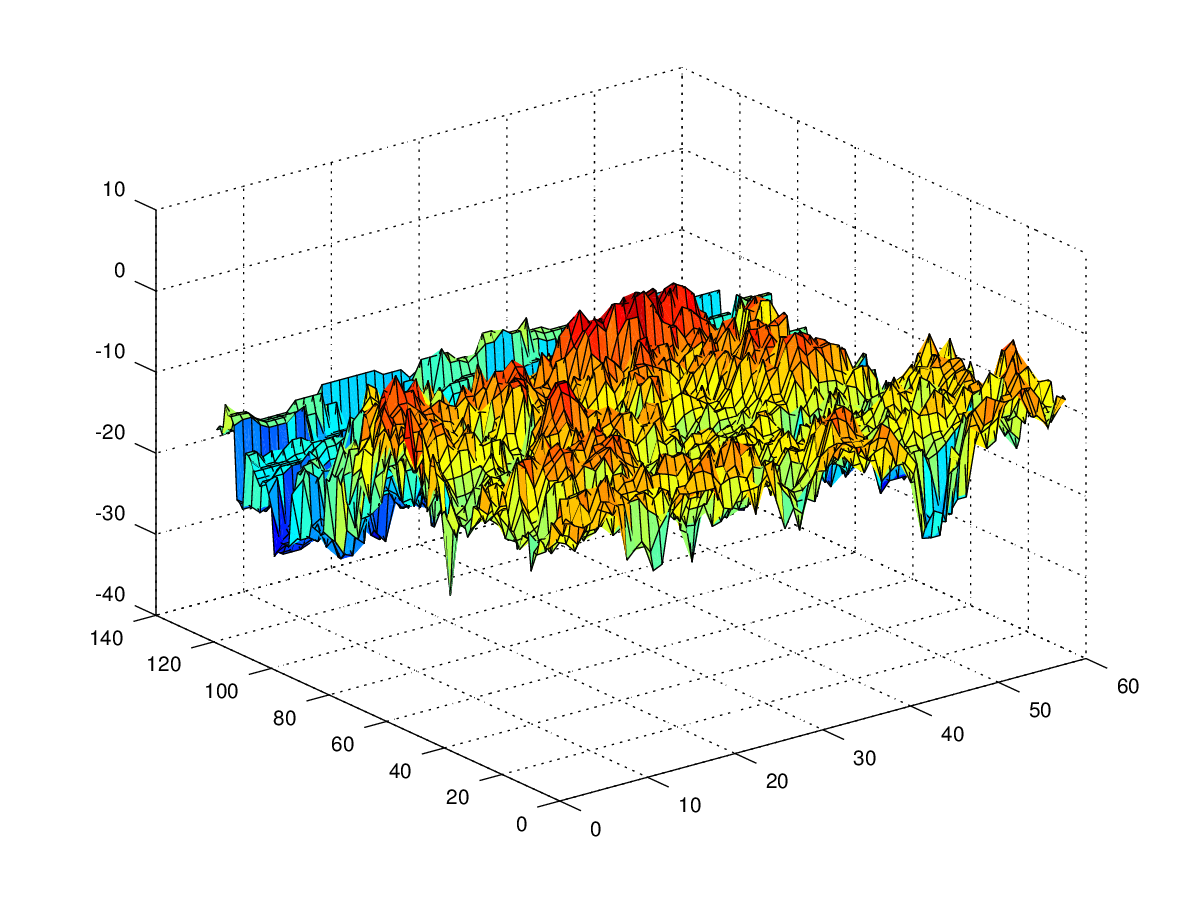
\includegraphics[scale=.3]{images/boostrawoutput}
  \caption{\em Gráficos obtenidos por la detección de la misma imagen sin la transformación en probabilidad, a la izquierda el resultado obtenido con SVM, a la derecha el resultado obtenido con Adaboost}  
  \label{fig:rawoutput}
\end{figure}


Los resultado obtenidos en esta etapa sin realizar la normalización no son muy buenos indicadores de sensibilidad espacial, ni tampoco son buenos resultados para realizar un post-procesamiento (la localización de peatones) de manera sencilla. Aparte del los gráficos obtenidos a partir de las matrices resultado (ver figura~\ref{fig:rawoutput}) se pueden observar la respuesta en la imagen para tener una idea de cómo es que se ve la detección sobre cada imagen. Un ejemplo de esto es la figura~\ref{fig:resultadoenimagen} en la cual se muestra el resultado en color sobre el peatón. Las detecciones con respuestas demasiado pequeñas o cero fueron eliminadas para ilustrar de mejor forma el fenómeno.

\begin{figure}[htc]
  \centering
  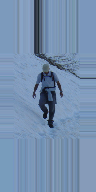
\includegraphics[scale=1]{images/imgorig}
  
\includegraphics[scale=1]{images/resultadosobreimagen}
  \caption{\em A la izquierda imagen original, a la derecha resultados obtenidos marcados sobre la imagen.}  
  \label{fig:resultadoenimagen}
\end{figure}


\subsection{Mapeo de probabilidades}

Como ya se mencionó anteriormente, se realizó un proceso de normalización de la salida tanto para SVM como para Adaboost. En este punto a todos los valores de cada matriz resultado se le aplicó la ecuación~\ref{eq:sigmoid} obteniendo de cada una de ellas una matriz resultado normalizada que permite ahora comparar directamente entre Adaboost y SVM además de facilitar considerablemente la etapa de post-procesamiento. En otras palabras lo realizado fue mapear la salida de los clasificadores a probabilidades.

\begin{figure}[htc]
  \centering
  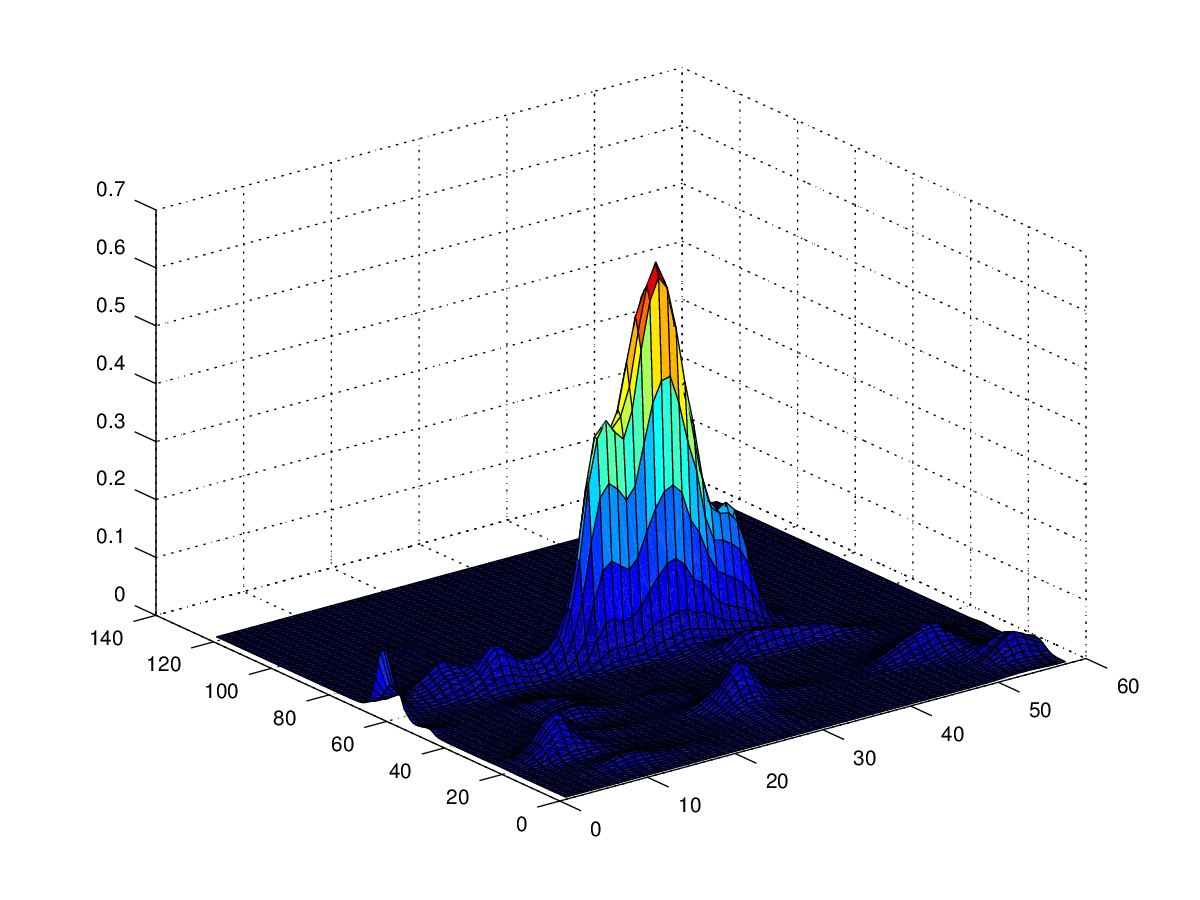
\includegraphics[scale=.3]{images/svmoutput}
  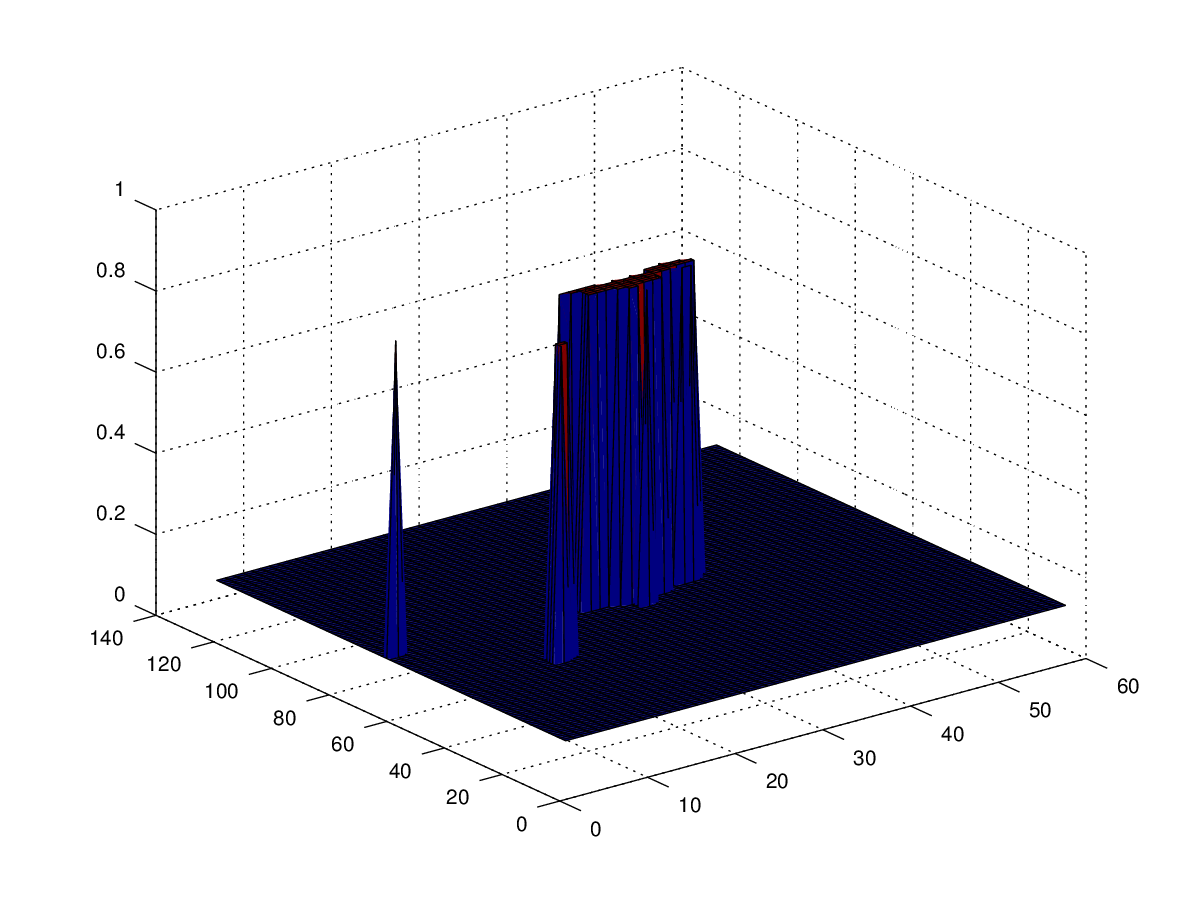
\includegraphics[scale=.3]{images/boostoutput}
  \caption{\em Gráficos obtenidos por la detección de la misma imagen con la aplicación de la normalización transformando el resultado en  probabilidad, a la izquierda el resultado obtenido con SVM, a la derecha el resultado obtenido con Adaboost}  
  \label{fig:output}
\end{figure}

Luego del mapeo en probabilidades los resultados están listos para realizar el cálculo de la sensibilidad espacial.

\subsection{Cálculo de las métricas de sensibilidad espacial}

El cálculo de las métricas se realizó de dos formas diferentes ya que esto permite comparar la sensibilidad al cálculo de la métrica y obtener información extra.

Con la primera forma de obtención se realizó un promedio de todas las matrices obtenidas con cada clasificador y se calculó el valor de las métricas a la matriz resultante de cada promedio. En otras palabras se generaron ocho matrices que representan las detecciones promedio para cada clasificador en el set de datos. Esta forma de calcular permite observar visualmente el fenómeno de la sensibilidad espacial y entrega información adicional sobre la detección en general.

La segunda forma de realizar el mismo cálculo es aplicar la métrica a cada matriz resultado de un mismo clasificador por separado y luego promediar todos los valores obtenidos. Esta segunda forma permite calcular de forma más sencilla otras medidas como la desviación estándar.

El proceso en particular de la métrica consiste en el cálculo de las diferencias de la matriz resultado con el modelo y luego maximizar los errores los que tendrán una mayor ponderación en la medida que los puntos evaluados se alejan del objeto a detectar, el cual en este caso se encuentra en el centro de la matriz.

\section{Resultados obtenidos}
\label{eval:resultados}

A continuación se ejemplificarán brevemente todos los resultados obtenidos del proceso para los dos tipos de clasificadores evaluados ya que se revisarán en detalle en el capítulo~\ref{cap:analisis} en el cual se realizará el análisis comparativo. Producto de este proceso de evaluación se obtuvieron una gran cantidad de resultados que, en particular, son de dos tipos: resultados gráficos y resultados numéricos. En esta sección se expondrán ejemplos de los resultados gráficos obtenidos, además de indicar una referencia a la forma en que fueron obtenidos. Los resultados numéricos serán presentados y evaluados en el capítulo~\ref{cap:analisis} a continuación.

\subsection{Resultados Gráficos}

Los resultados gráficos en general fueron obtenidos utilizando el paquete GNU Octave (similar al comercial MATLAB). Para facilitar el proceso se utilizó el formato que Octave utiliza para leer matrices de archivo de texto plano. Este formato considera una cabecera donde se indica el tipo de data, nombre de la variable, número de filas y número de columnas y a continuación la información de la matriz.

El primer tipo de gráfico obtenido corresponde al gráfico sin procesar de la matriz resultado, eso es con los valores obtenidos directamente del SVM lineal o Adaboost sin pasar por el proceso de normalización, algunos ejemplos de esto ya fueron expuestos anteriormente en la figura~\ref{fig:rawoutput}, sin embargo, esos no son los únicos ejemplos ya que para cada imagen detectada  es posible obtener uno de estos gráficos por lo que en la figura~\ref{fig:rawex}, se podrá encontrar más ejemplos de estas gráficas en el anexo~\ref{cap:gre}.

\begin{figure}[htc]
  \centering
  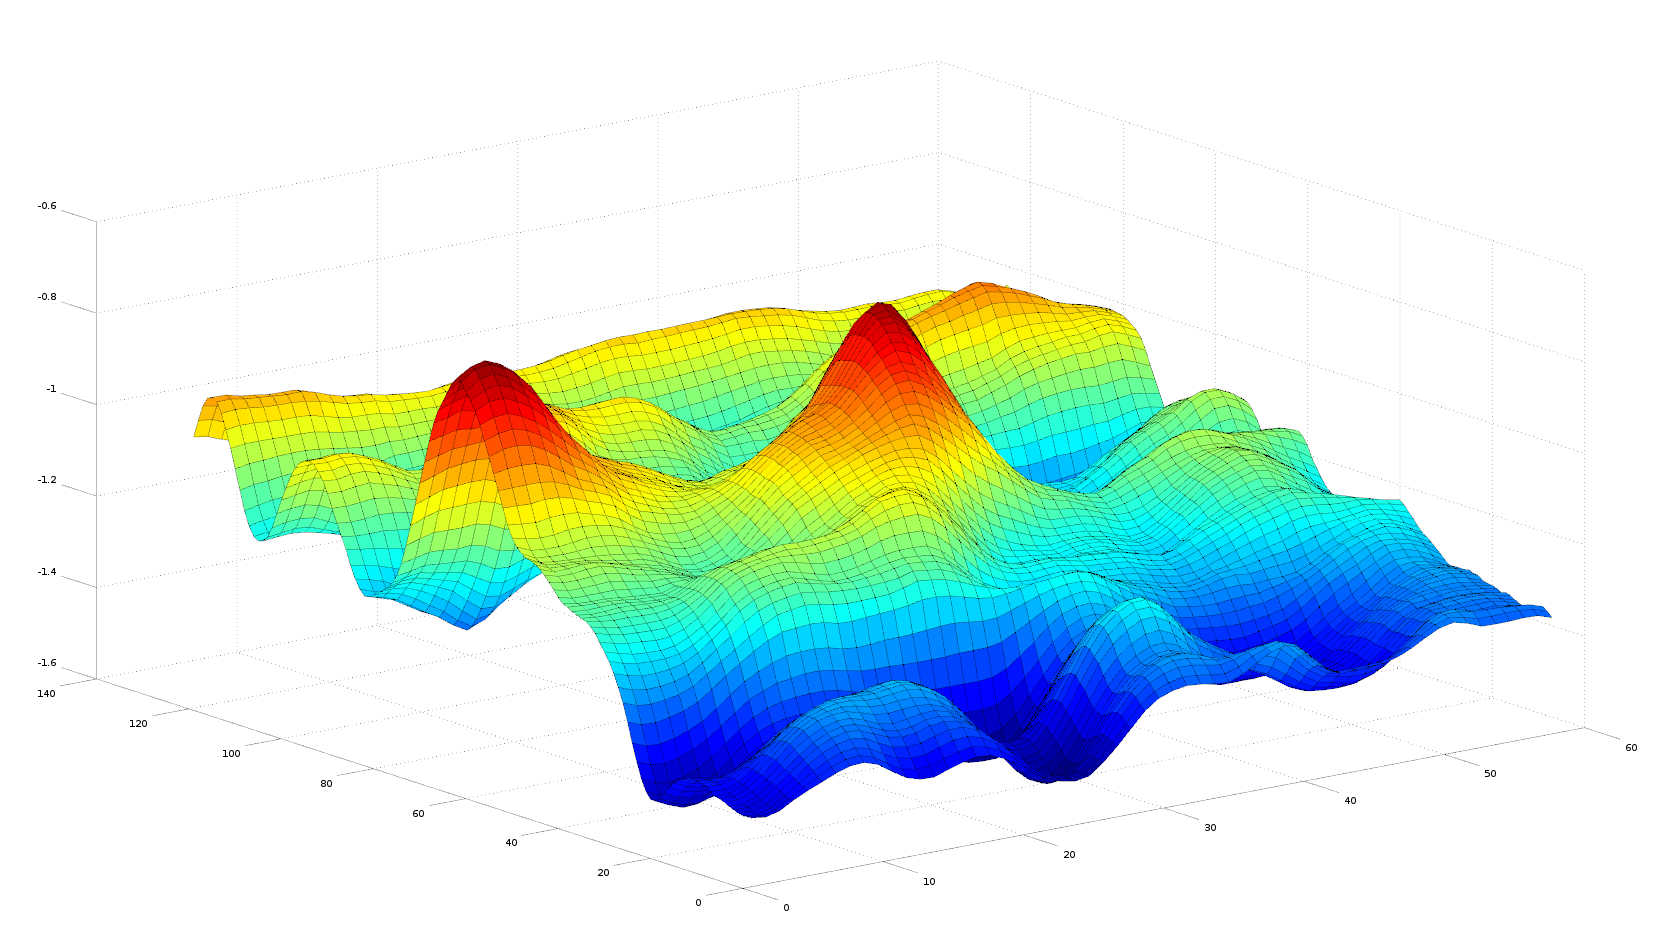
\includegraphics[scale=.1]{images/raw/1}
  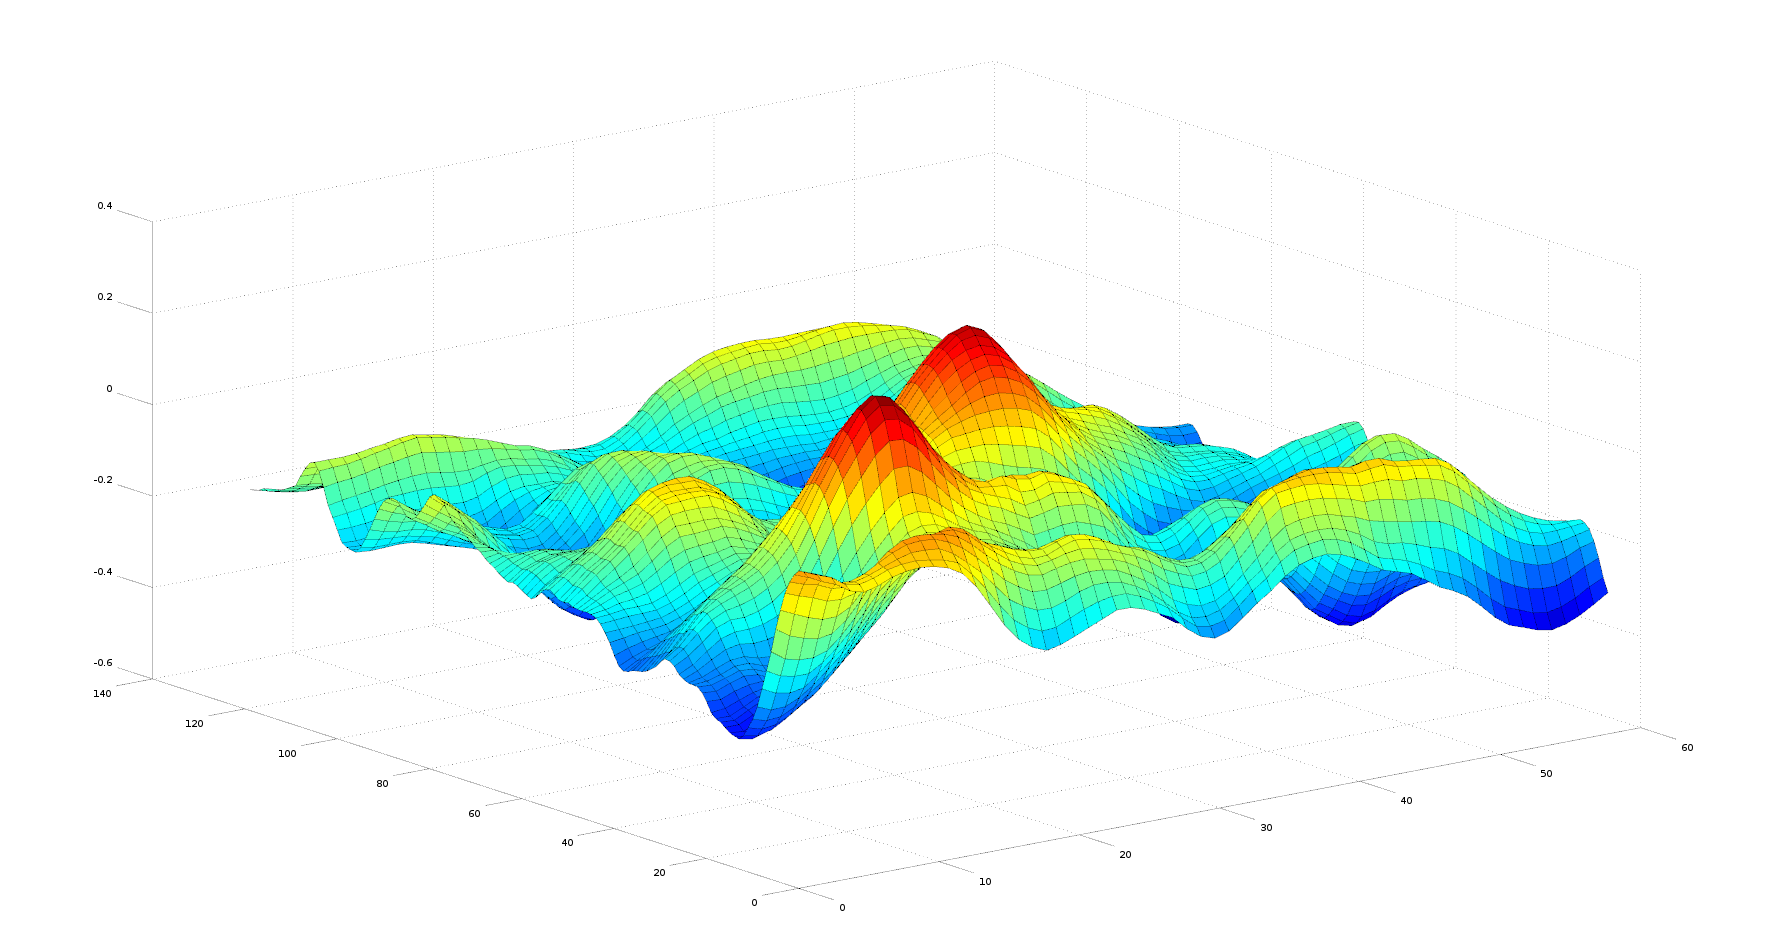
\includegraphics[scale=.1]{images/raw/2}
  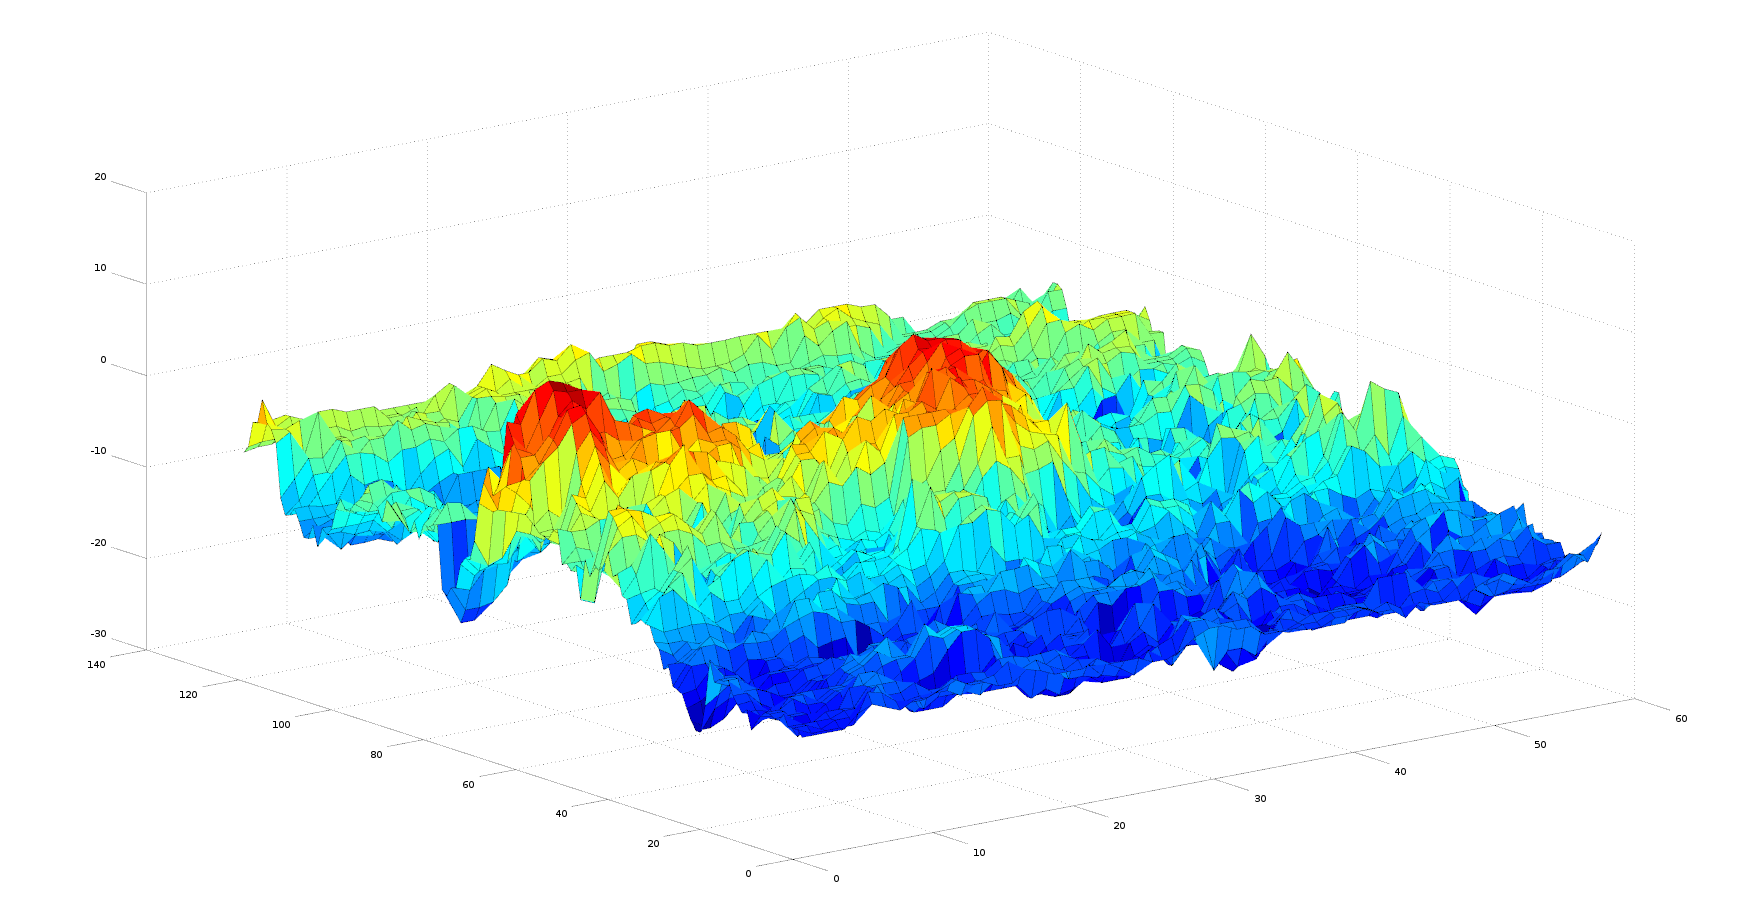
\includegraphics[scale=.1]{images/raw/3}
  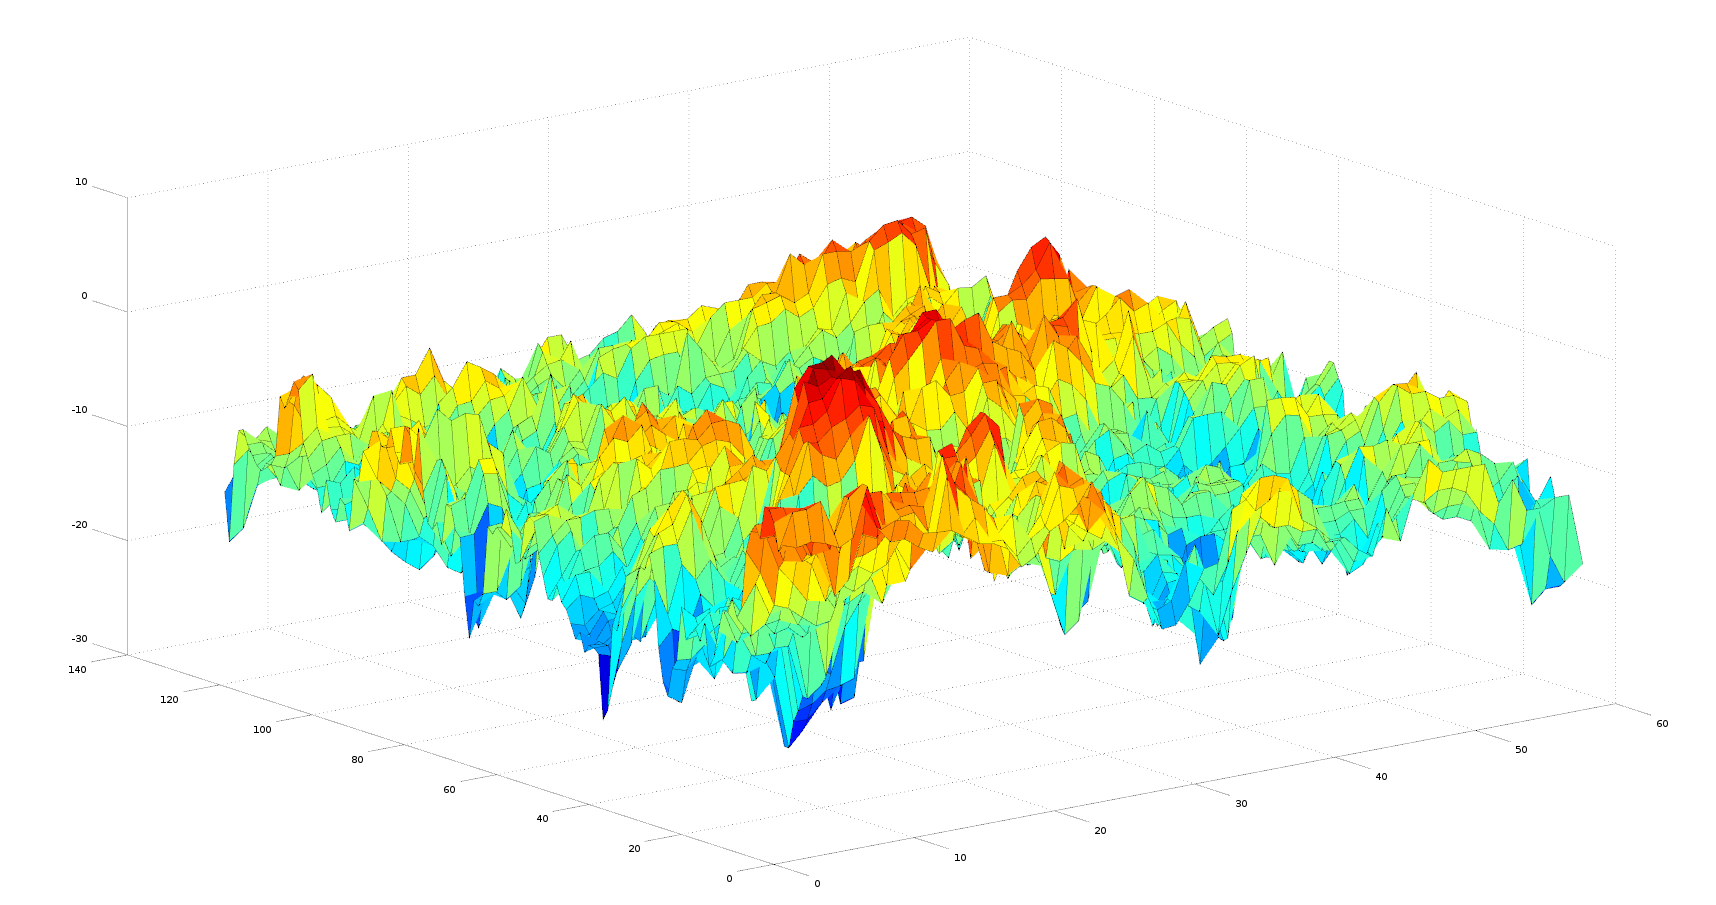
\includegraphics[scale=.1]{images/raw/4}
  \caption{\em Ejemplo de gráficos con resultados la matriz desnormalizados (sin pasar por el proceso de normalización), arriba gráficos obtenidos con SVM lineal, abajo gráficos obtenidos con Adaboost}  
  \label{fig:rawex}
\end{figure}

Un segundo tipo de gráfico obtenidos son los gráficos de matriz resultado con la normalización aplicada, este tipo de gráficos son en general el siguiente paso respecto de los gráficos sin procesar son el resultado de mapear los valores de cada matriz en los valores obtenidos pos la función sigmoidal que permite la normalización. Ejemplos de estos gráficos al igual que con los anteriores ya fueron expuestos en la figura~\ref{fig:output}. Sin embargo, es importante mostrar algunos ejemplos diferentes en la figura~\ref{fig:sigex}. Es necesario mencionar que estos ejemplos corresponden directamente con los de la figura~\ref{fig:rawex} pues fueron obtenidos a partir de la mismas imágenes.


\begin{figure}[htc]
  \centering
  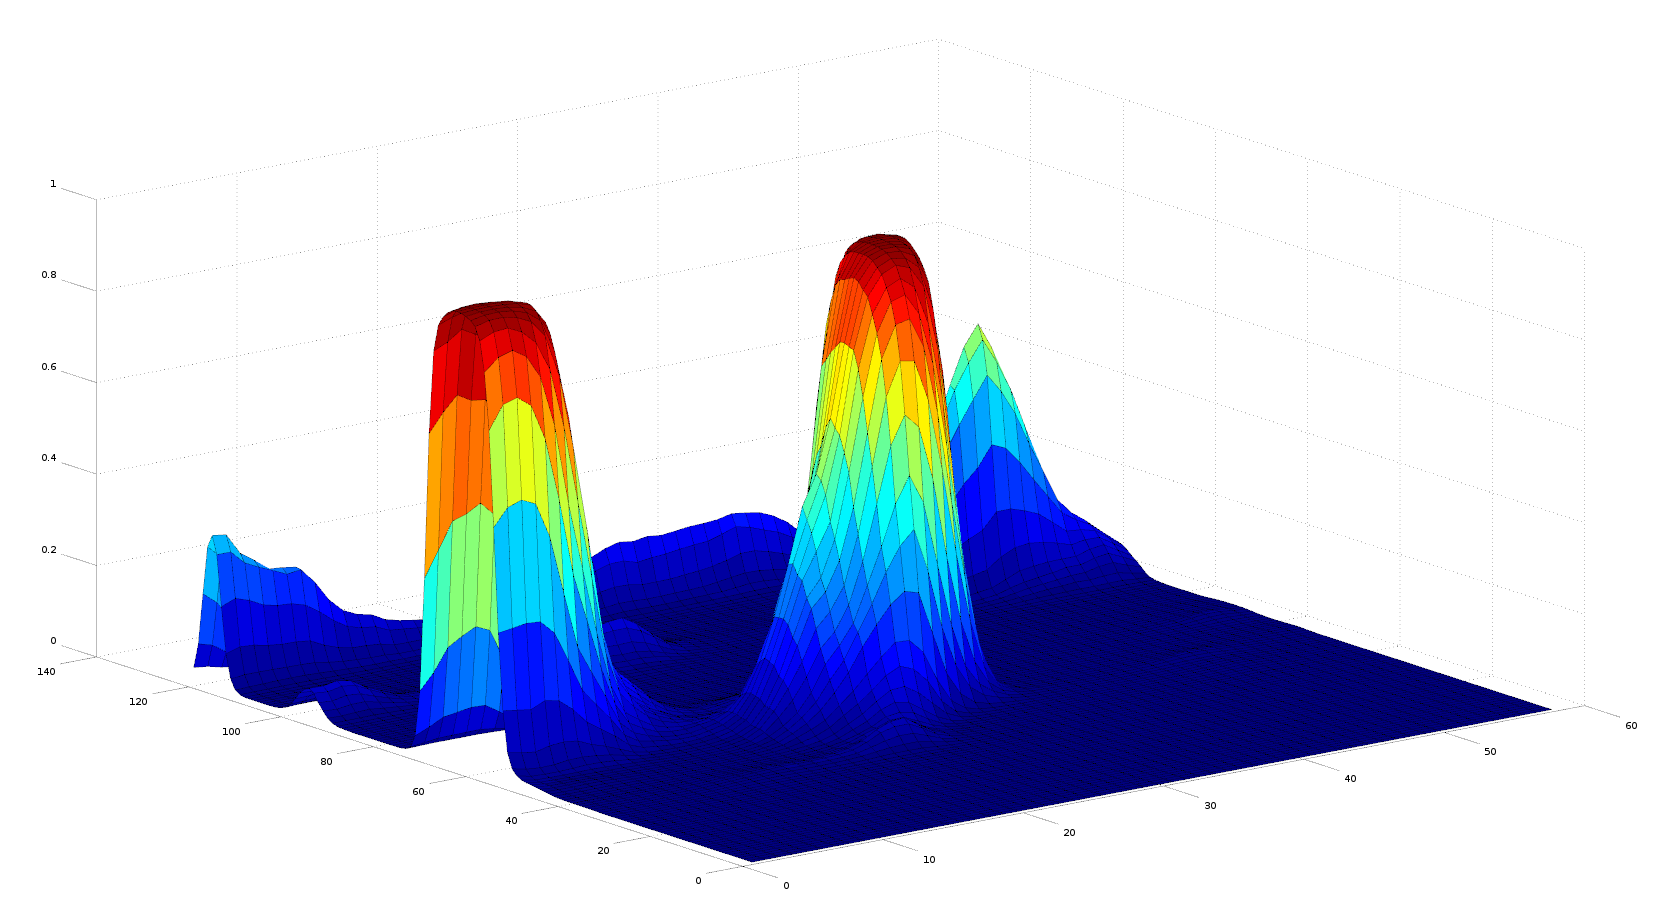
\includegraphics[scale=.1]{images/sig/1}
  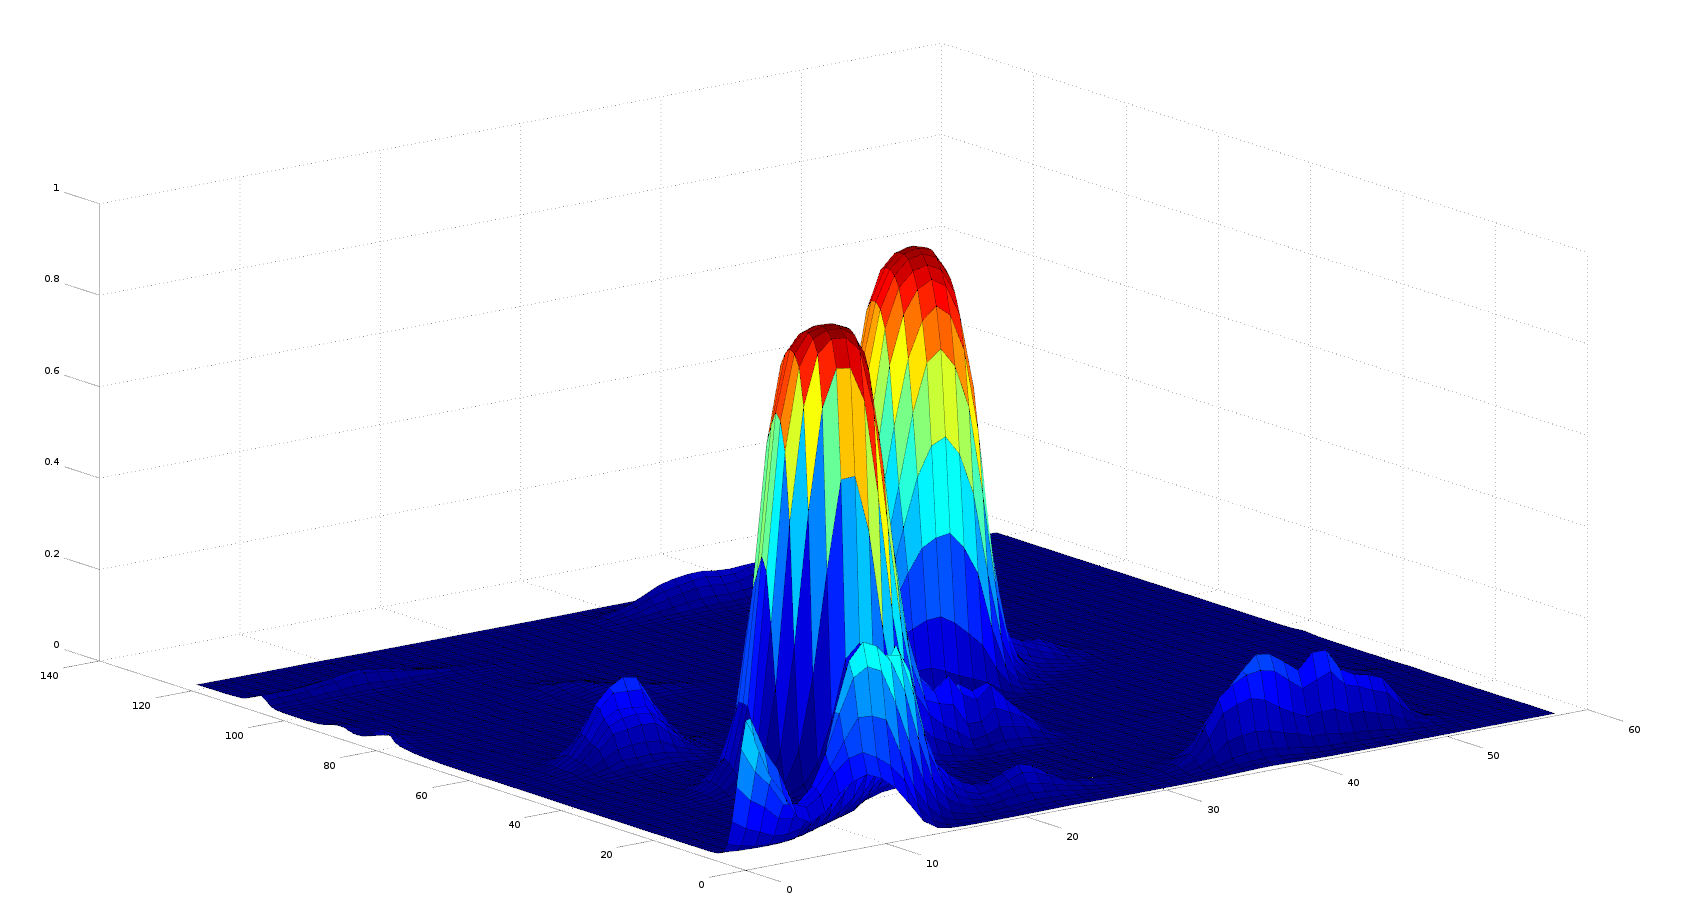
\includegraphics[scale=.1]{images/sig/2}
  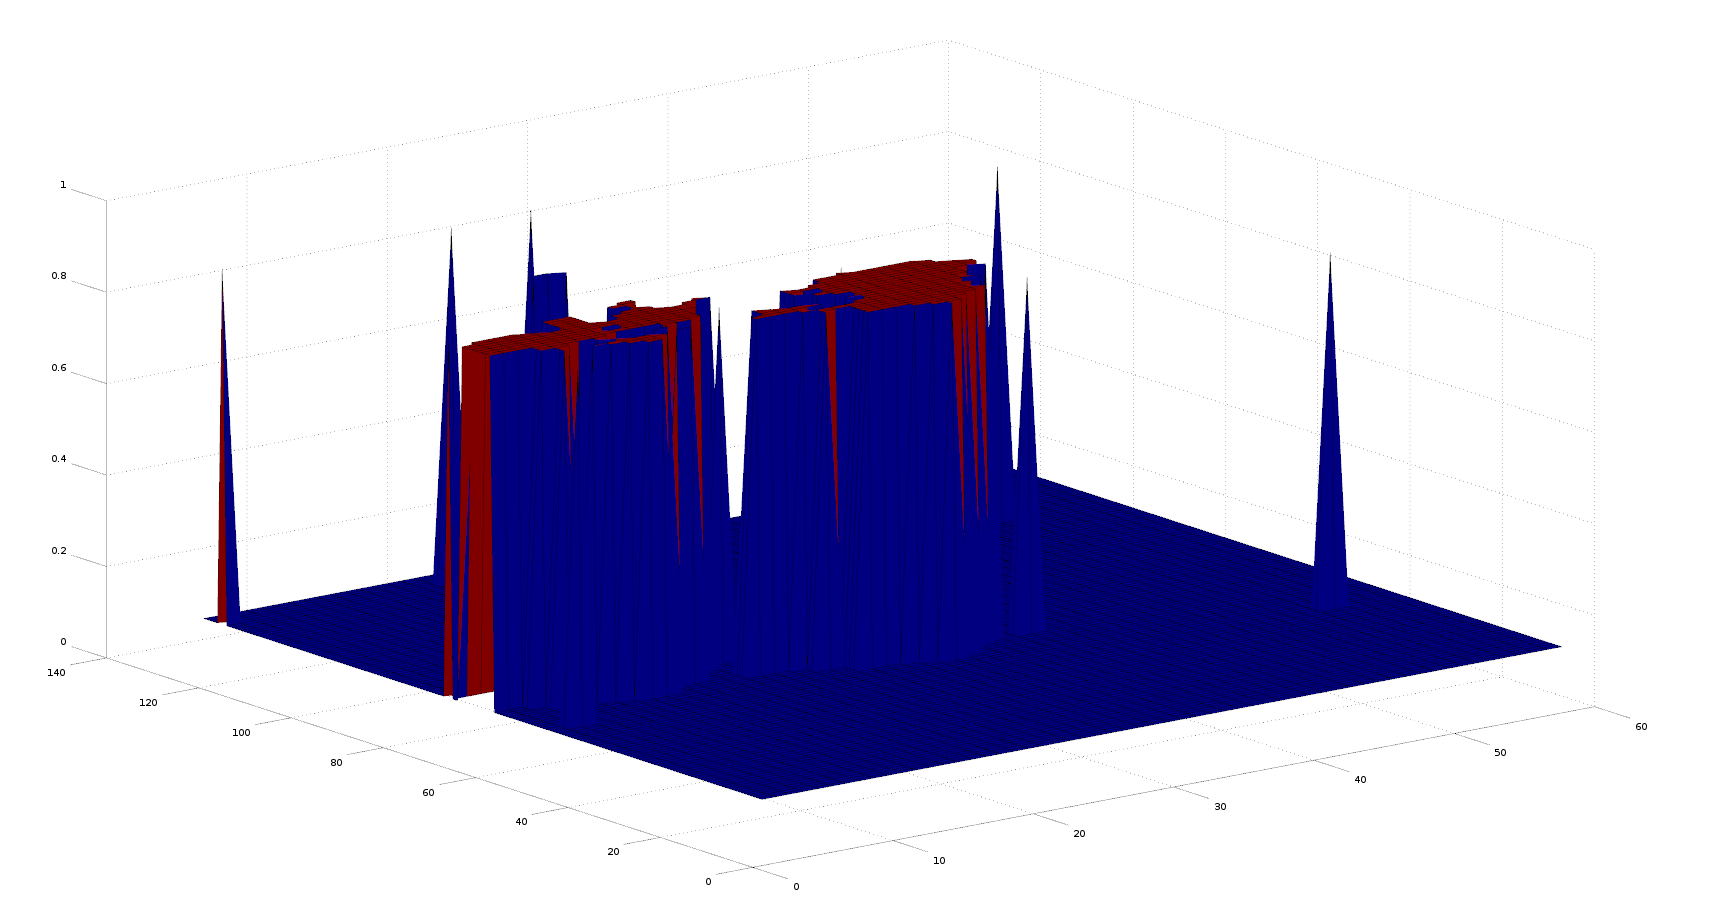
\includegraphics[scale=.1]{images/sig/3}
  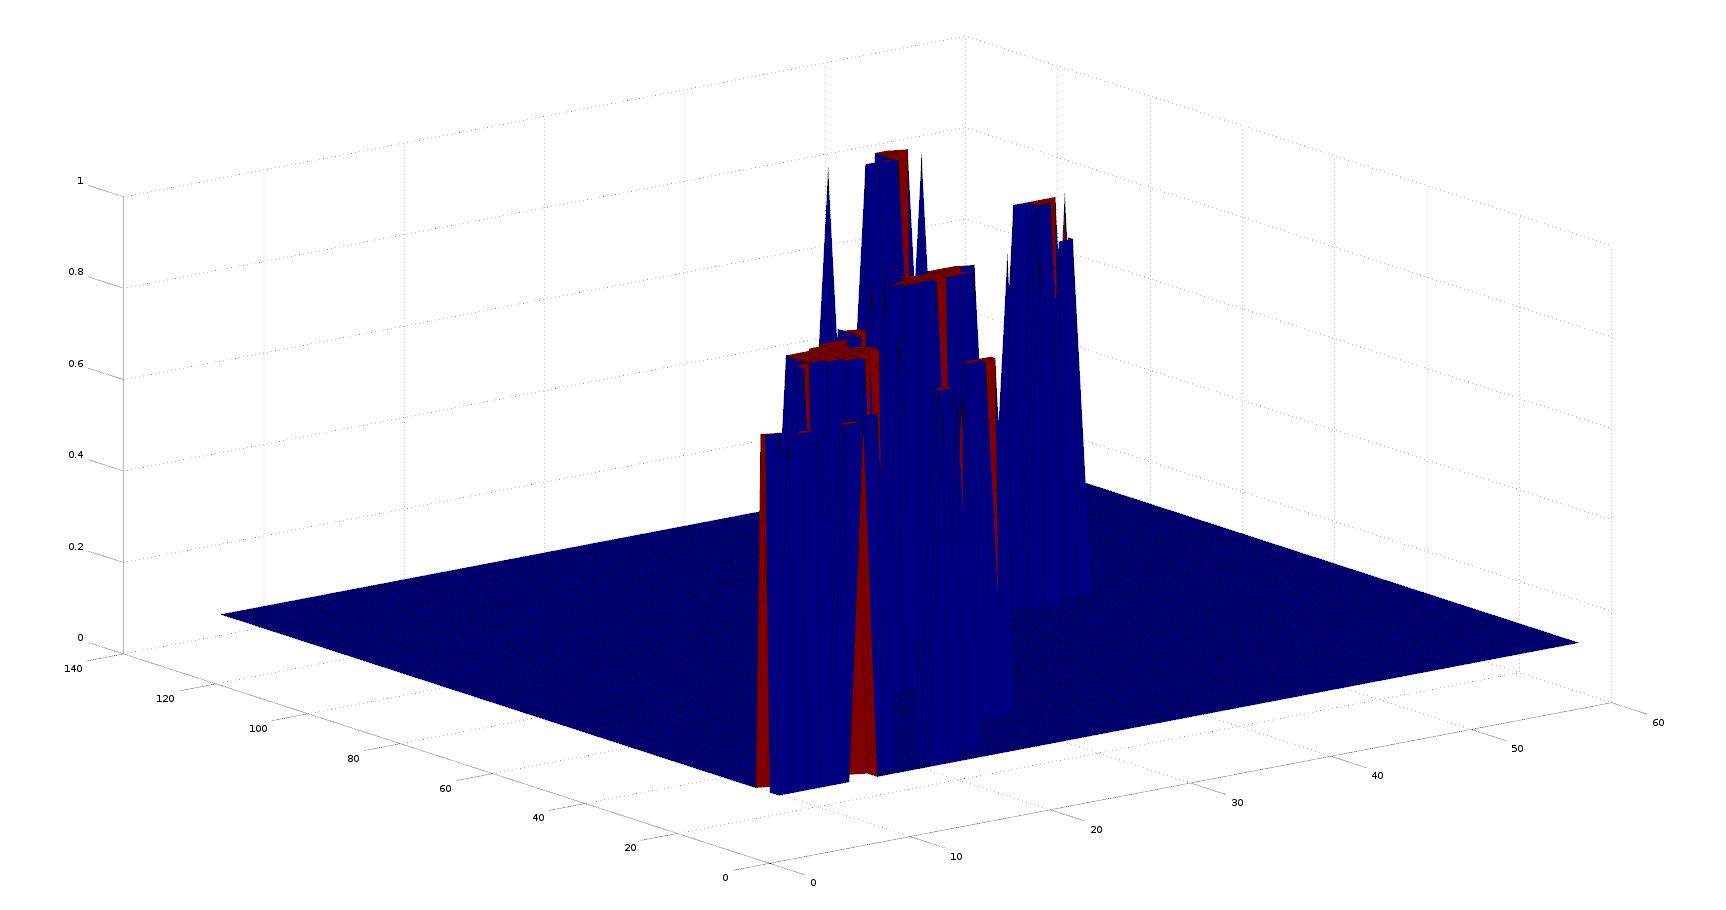
\includegraphics[scale=.1]{images/sig/4}
  \caption{\em Ejemplo de gráficos con resultados la matriz desnormalizados (sin pasar por el proceso de normalización), arriba gráficos obtenidos con SVM lineal, abajo gráficos obtenidos con Adaboost}  
  \label{fig:sigex}
\end{figure}

El último tipo de gráfico en tres dimensiones es el obtenido con el promedio de las matrices. Estos gráficos representan de mejor forma la detección general realizada por el clasificador a todo el conjunto de datos, analizando este tipo de gráficos es posible describir comportamientos generales que se pueden luego aplicar en otros contextos. En la figura~\ref{fig:soutput}~se puede observar ejemplos de estos gráficos que en el siguiente capítulo se analizarán en detalle.

\begin{figure}[htc]
  \centering
  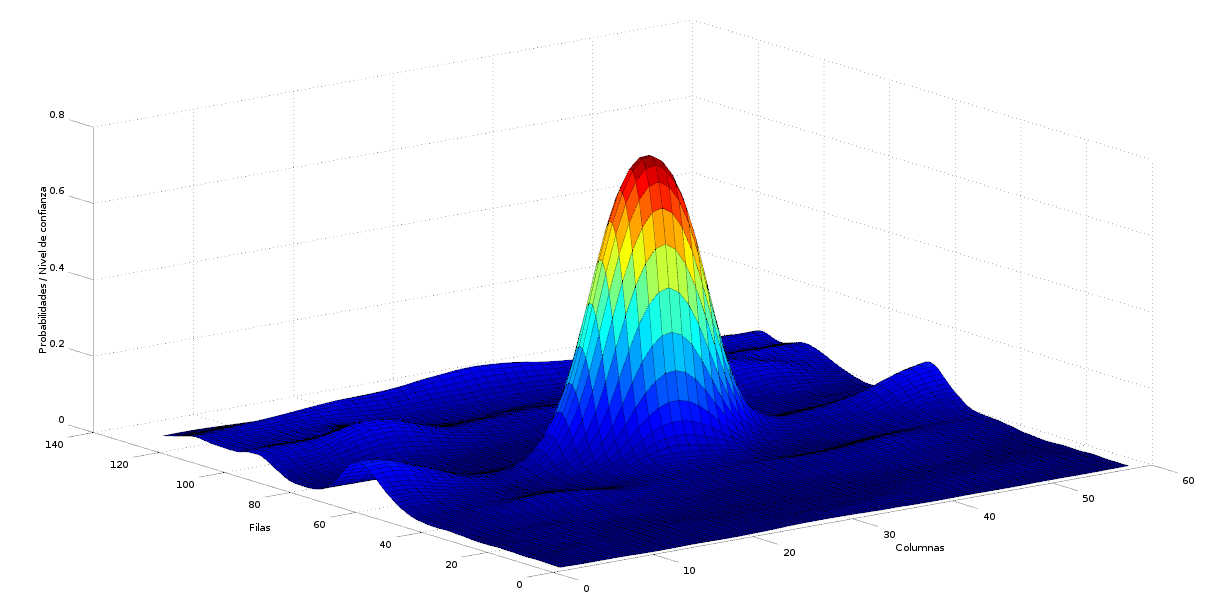
\includegraphics[scale=.16]{images/meansvmout32}
  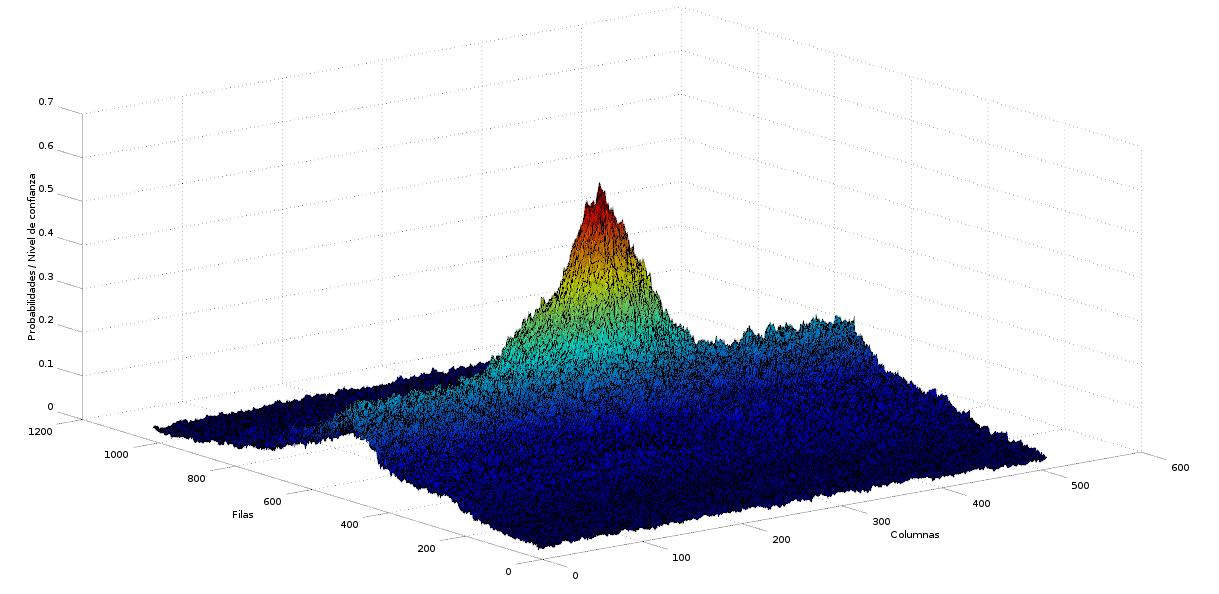
\includegraphics[scale=.16]{images/meanboostout256}
  \caption{\em A la izquierda, gráfico de sensibilidad espacial promedio de una SVM lineal con una ventana de detección de 32x64px. A la derecha, gráfico de sensibilidad espacial promedio de Adaboost con una ventana de detección de 256x512px}  
  \label{fig:soutput}
\end{figure}


Dado el tamaño de estos gráficos es muy difícil colocar indicaciones en los ejes que ayuden a su interpretación,  por lo que a continuación se explican sus significados, pero teniendo en cuenta que la interpretación de cada eje es la misma para todos los gráficos tridimensionales expuestos en este documento.

\begin{itemize}
\item Eje x. Es el que se observa en línea oblicua desde el centro hacia la derecha y representa las columnas de la imagen.
\item Eje y. Es el que se observa en línea oblicua desde el centro hacia la izquierda y representa las filas de la imagen.
\item Eje z. Es la elevación y representa la magnitud del valor de la detección.
\end{itemize}

Otros resultados gráficos son aquellos obtenidos de la proyección de las matrices hacia sus ejes. Un ejemplo de esos son los gráficos en la figura~\ref{fig:proyecciones} en el capítulo~\ref{cap:metricas}. Estos gráficos no entregan mayor información que los tridimensionales por lo que no son utilizados como herramienta comparativa. Sin embargo es posible encontrar ejemplos de estos gráficos en el anexo~\ref{cap:gre}.

\section{Implementación}

Para la implementación del proceso de evaluación se utilizó principalmente los lenguajes de programación C++ y Python. Para guiar la implementación se utilizó una adaptación de la metodología de software XP,                  La cual se explicará a continuación.

\subsection{\textit{Extreme Programming} aplicado a equipos unipersonales}

En la sección anterior se ha explicado resumidamente en qué consiste la metodología de \textit{Extreme Programming}. Sin embargo, dado el contexto del desarrollo de la solución para este trabajo, esta metodología no podía funcionar directamente \textit{out-of-the-box} para el contexto en el cual se debía realizar tal desarrollo. La razón principal es que XP originalmente se orienta a equipos, compuestos por al menos dos personas (una de sus prácticas principales es la programación por pares), y el equipo de desarrollo para este caso sólo estuvo compuesto de una sola persona. No obstante, la mayor parte de la metodología fue útil para los propósitos planteados; por tanto solo era necesario encontrar una adaptación que permitiera a un individuo aplicar los principios de XP en su labor.
	En el sitio web \cite{xpforone2006} muestra una forma en la que XP puede adaptarse para funcionar con un equipo unipersonal. Si bien en este caso los requerimientos no cambian de forma radical, durante el desarrollo de la solución podían presentarse imprevistos u obstáculos inesperados que gracias a la metodología podían salvarse rápidamente en comparación a otras metodologías más tradicionales. Se utilizaron Historias de Usuario para definir los requerimientos asociados a la solución y para programar el desarrollo, se utilizó una lista de tareas (\textit{To-Do List}) que priorizaba las Historias de Usuario según las necesidades del cliente. La prioridad en este caso fue definida según dos criterios principales.
\begin{itemize}
\item Según el valor que aportara la implementación de las funcionalidades a la solución final. Aquellas funcionalidades “principales” de la solución recibían mayor prioridad que las funcionalidades anexas. Este criterio tiene mayor prioridad.
\item Según las dependencias implícitas en el desarrollo. Si existen historias de usuario que implican el desarrollo de funcionalidades de valor similar dependientes una de la otra, recibe mayor prioridad la historia de usuario que implica el desarrollo del componente del cual depende la otra historia de usuario.
\end{itemize}
	
Existen otros elementos de la metodología XP que se cumplen inmediatamente en un equipo unipersonal. Si el trabajo es desarrollado por una sola persona, la comunicación es inmediata sobre sí misma, más aún si ella misma es el cliente (aunque sin dejar de lado los posibles cambios en los requerimientos causados por factores externos, tales como las asesorías de terceros sobre la solución en implementación). Asimismo, la mantención de estándares en la programación y la documentación del código se hacen ya no con el fin de que otros miembros del equipo puedan comprender e intervenir en el código, sino que el mismo desarrollador siga una estructura ordenada y entendible, por sí mismo y por terceros que puedan revisar el código generado.


\section{Conclusiones del capítulo}
% ***SAV falte

En este capítulo se ha descrito el proceso de evaluación de la sensibilidad espacial que se aplica a los clasificadores considerados, que consta de siete etapas, Ajuste del set de datos, esto es, adaptar las imágenes del set de datos original para que fueran utilizadas por los clasificadores en escalas distintas a la original. Extracción de características, las que generan matrices de vectores de características producto de la aplicación de HOG. Entrenamiento de los clasificadores utilizando las matrices de características y las etiquetas peatón / no peatón. Entrenamiento del sigmoide que permite normalizar las salidas de los clasificadores, transformándolas a probabilidades, utilizando el método de \cite{Platt1999}, con la mejora propuesta por \cite{Lin2000}. Detección en la vecindad, moviendo la ventana deslizante prácticamente píxel a píxel, con el fin de que el ejercicio de detección reflejara fielmente los resultados de cada clasificador en las vecindades de los objetos a detectar, y por ende, poder determinar con mayor precisión la sensibilidad espacial de cada uno de éstos. Mapeo a probabilidades, esto es, aplicar el sigmoide entrenado a las salidas de los clasificadores, transformando efectivamente sus salidas en probabilidades, obteniendo gráficos que permiten apreciar el grado de detección de cada clasificador con respecto al objeto y a su entorno, permitiendo el cálculo de la sensibilidad espacial, así como también su estimación visual en comparación al caso ideal. Cálculo de las métricas de sensibilidad espacial que permiten determinar qué clasificador es más sensible espacialmente con respecto a otro(s). 
El proceso de evaluación permitió la generación de distintos gráficos que permitían apreciar los resultados generados por los clasificadores y la información referente a la sensibilidad espacial de cada uno de éstos. Este proceso fue implementado mediante \textit{Extreme Programming} aplicado a un equipo unipersonal, con la ayuda de los lenguajes C++ y Phyton, además de bibliotecas como OpenCV.
